% Translated to Java
\chapter{Elementary Programming}
\label{sec:elementary}

Here are some basic programming knowledge. I hope you have seen some of the concepts in this chapter already on other occasions. This is a good opportunity to recap, or to familiarise yourself with C++ if you are not a C++ programmer. I would like to stress that most programming concepts discussed in this piece of notes are transferable to most other programming languages.

% Translated to Java end 

\subsection*{Further resources (Ch 1-2)}
\addcontentsline{toc}{section}{Further resources (Ch 1-2)}
\link{https://www.youtube.com/watch?v=tvC1WCdV1XU&list=PLAE85DE8440AA6B83}{Bucky's C++ Programming Tutorial} (a YouTube playlist) covers most things that you need to know about C++, and also most of the things in this chapter. You only need to watch the first 20-30 videos, as it goes too deep in the later episodes.

\subsection*{Practicing at home}
Practicing is very important. For example, one of the things I would do back then is to remove the one or two lines that I didn't understand in the materials, and see how they affected the program by printing out the values of the variables at different times. 

Refer to \cref{sec:settingup} on how to run C++ code on your own device.

\subsection*{Structure of a C++ program}
\begin{lstlisting}
//First include the libraries that you are going to use
#include <iostream> 

//A weird line of code that you have to remember every time you write a C++ program.
using namespace std;

int main(){
    cout << "Hello world" << endl;
    return 0;
}
\end{lstlisting}

The main function is the point of entry of the program.

You need to add a semicolon at the end of every statement or else the compiler will shout at you. 

Comments are denoted as \texttt{//}.

\subsection*{Variables}

\textit{A variable is just like an empty box. You can store stuff in it. Technically, it is nothing but a name given to a computer memory. That's it, now go spend rest of your life deciding the perfect variable name.} \footnotecite{variableig}

It is important to distinguish between initialisation of the variable and reassignment of the variable.

\begin{lstlisting}
int score = 70; //initialisation
score = 80; //reassignment
\end{lstlisting}

You have to specify the type of variables when initialising them in C++. Each variable can only be used to store data of a single type. Common types include \code{int} for integers, \code{double} for numbers with decimal places i.e. \textbf{floating point numbers}, \code{char} for one character, and \code{bool} for \code{true} or \code{false} i.e. \textbf{Booleans}. 

It is not compulsory to give an initial value to a variable. If you do not do so, it will be a random number until you reassigns it.

\begin{lstlisting}
int score = 70; //initialisation
cout << score << endl; //unexpected value
score = 80; //reassignment
cout << score << endl; //80
\end{lstlisting}

You can see a list of datatypes that C++ offers in \cref{sec:primarydtypes} and we will dedicate our full attention to datatypes and Boolean operators in \cref{sec:dtypes}.

\subsection*{Operators}
We can perform arithmetic operations like \code{+ - * /} on numbers, \code{/} will only return a floating point number when at least one of its arguments are floating points. Otherwise, it will \textbf{truncate} the number to an integer. % not round down due to negative arguments

We can also calculate the remainder of a division using the \code{\%} operator. \code{a\%b} computes the remainder of \code{a} when divided by \code{b}. We assume \code{a} is a non-negative integer and \code{b} is a positive integer. It will give an error when supplied with floating point arguments. Its behaviour for integers outside its range is not well-defined.

There are also some operators that works on Booleans including \code{!} for NOT, \code{\textbar\textbar} for OR and \code{\&\&} for AND. We will look into them in detail in \cref{sec:booleanop}.

\subsection*{Console I/O}

It is important to be able to visualise the result of our program and to interact with our program.

\texttt{cout} stands for Console OUTput. You put the things (variable or strings - sequence of characters) that you want to print after the \texttt{cout} keyword, separated by \texttt{<<}. The \texttt{endl} keyword inserts a newline character. Remember to use double quotes for strings.

\texttt{cin} stands for Console INput. You put variables that you would like the output to be stored in after the \texttt{cin} keyword, separated by \texttt{>>}. 

The direction of the arrows may be hard to remember, but it is intuitive once you associate them with the direction of information flow. You want text to flow towards the screen (the \texttt{cout} keyword) when you are outputting, and towards the variables when asking for user input.

\begin{lstlisting}
cout << "What is your score? ";
int score;
cin >> score;
cout << "Your scored " << score << " in this paper." << endl;
\end{lstlisting}

\section{Conditionals}

More complicated code do not just go like a straight line, the programming constructs below allow the code to do different things based on the current state of the machine or based on different user input.

\subsection{\texttt{if} statements}

The simplest form of conditionals.

\begin{lstlisting}
int score;
cin >> score;
if(score >= 70){
    printf("Good job.\n");
}else if(score >= 40){
    printf("You got a pass.\n");
}else{
    printf("You failed.\n");
}
\end{lstlisting}

\subsection{\texttt{switch case}} 

{\footnotesize (Of less importance)}

Just looks neater when you are testing on the same variable multiple times. You can of course use if else if else if... 

Note that it only works for int and char, and only equality tests are allowed. For example, the above example on scores could not be replaced using switch case.

Also note that the \textbf{\texttt{break}} keyword is necessary to quit the switch statement, or else it will run the default clause after the \texttt{case} clause.

\begin{lstlisting}
char x;
cin >> x;
switch(x){
    case 'z':
        cout << "It is the last letter of the alphabet." << endl;
        break;
    //this is how you do multiple equality tests
    case 'a':
    case 'e':
    case 'i':
    case 'o':
    case 'u':
        cout << "It is a vowel." << endl;
        break;
    //equivalent to the else clause
    default:
        cout << "It is not a vowel." << endl;
        break;
}
\end{lstlisting}

% Translated to Java

\section{Arrays}
\label{sec:arrayintro}
Arrays store sequences of data of the same type.

\if\proglang1
\begin{lstlisting}
int[] x = {3,1,4,1,5,9,2,6};

System.out.println(x[0]); //3 
System.out.println(x[4]); //5
System.out.println(x[7]); //6 (last element)
System.out.println(x[8]); //Error 
\end{lstlisting}
\else
\begin{lstlisting}
int x[8] = {3,1,4,1,5,9,2,6};
//alternatively: int x[] = {3,1,4,1,5,9,2,6}; length of array can be omitted as the compiler can derive it from the right hand side

cout << x[0] << endl; //3 
cout << x[4] << endl; //5
cout << x[7] << endl; //6 (last element)
cout << x[8] << endl; //unexpected value (Why?)
\end{lstlisting}
\fi

We call the things stored in the array \textbf{elements}. We distinguish different elements using \textbf{index}. The index \textbf{starts from 0}, and ends at $n-1$, where $n$ is the length of the array. The \textbf{length} of the array refers to the maximum number of elements that the array can store, based on the memory allocated when it is \textbf{initialised}. We cannot change the length of the array normally.

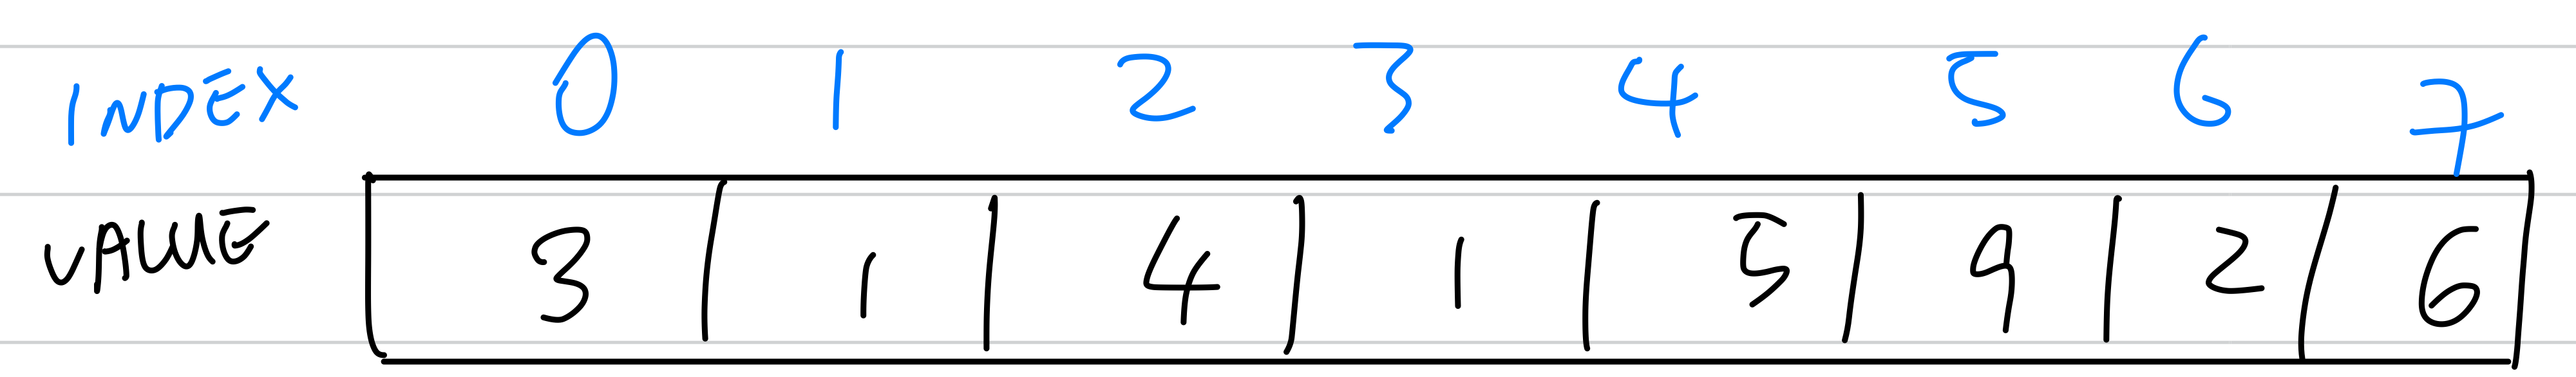
\includegraphics[width=12cm]{images/ch2-arrayindex.png}

There are two ways of initialising arrays. The first way is to hard-code the elements in the array. The length of the array is inferred by the number of elements given, and it cannot be extended afterwards.

\if\proglang1
\begin{lstlisting}
int[] x = {3,1,4,1,5,9,2,6};
\end{lstlisting}
\else
\begin{lstlisting}
int x[] = {3,1,4,1,5,9,2,6};
\end{lstlisting}
\fi

The second way is when you are not quite sure what the elements of the array are yet, but you must still supply the length of the array.

\if\proglang1
\begin{lstlisting}
int[] x = new int[8];
\end{lstlisting}
\else
\begin{lstlisting}
int x[8];
\end{lstlisting}
\fi

Arrays turn out to be a very important programming construct, and we would dedicate our whole attention to it in \cref{sec:arraychap}.
% Translated to Java end

\section{Loops}

More complicated programs often require the same bit of code executing multiple times, the use of loops allows us to write shorter code. (Of course there are many other uses of it but it is best understood by looking at examples and practice)

\subsection{\texttt{for} loops}
\label{sec:forloops}
Runs the body a specified number of times.

\begin{lstlisting}
int x[8] = {3,1,4,1,5,9,2,6};
int sum = 0;
for(int i = 0; i < 8; i++) { //loops i=0,1,2,3,4,5,6,7
    sum += x[i];
}
cout << sum << endl; //31
\end{lstlisting}

\begin{lstlisting}
int x[8] = {3,1,4,1,5,9,2,6};
int sum = 0;
for(int i = 7; i >= 0; i--) { //loops i=7,6,5,4,3,2,1,0
    sum += x[i];
}
cout << sum << endl; //31
\end{lstlisting}

\subsection{\texttt{while} loops}
Runs the body until the test is false.
\begin{lstlisting}
int x[8] = {3,1,4,1,5,9,2,6};
int sum = 0;
int i = 0;
while(i<8) { 
    sum += x[i]; //loops i=0,1,2,3,4,5,6,7
    i++;
}
cout << sum << endl; //31
\end{lstlisting}

\begin{lstlisting}
int x[8] = {3,1,4,1,5,9,2,6};
int sum = 0;
int i = 0;
while(i<8&&x[i]%2==1) { 
    sum += x[i];
    i++;
}
cout << sum << endl;
\end{lstlisting}

%4

\subsection{\texttt{do while} loops}
Runs the body until the test is false. The body will run at least once.

\begin{lstlisting}
bool emergency = false;
do{
    printf("EMERGENCY\n"); //will be printed
}while(emergency);
\end{lstlisting}

\begin{lstlisting}
bool emergency = false;
while(emergency){
    printf("EMERGENCY\n"); //will not be printed
}
\end{lstlisting}

This example yields the same result with while loops because the test is true initially, allowing the loop to run at least once.

\begin{lstlisting}
int x[8] = {3,1,4,1,5,9,2,6};
int sum = 0;
int i = 0;
do { 
    sum += x[i]; //loops i=0,1,2,3,4,5,6,7
    i++;
}while(i<8);
cout << sum << endl; //31
\end{lstlisting}

\subsection{Infinite loops}

If the test case is always true (there is nothing in the loop to make the test false). The loop is an infinite loop\index{infinite loop}, where the loop will not terminate (until resources are used up), and the remaining parts of the program can never be run. In this example, EMERGENCY will be printed forever nonstop.

\begin{lstlisting}
bool emergency = true;
while(emergency){
    printf("EMERGENCY\n");
}
destroy_world(); //will not be run
\end{lstlisting}

\subsection{\texttt{break}}
\label{sec:loopbreak}
\texttt{break} allows you to terminate the loop early.

\begin{lstlisting}
int x[8] = {3,1,4,1,5,9,2,6};
int sum = 0;
int i = 0;
while(i<8) { 
    sum += x[i];
    i++;
    if(sum >= 10) break;
}
cout << sum << endl;
\end{lstlisting}

% 14

\subsection{\texttt{continue}}
\label{sec:loopcontinue}
\texttt{continue} allows you to jump to the next iteration, skipping the rest of the current iteration early.

\begin{lstlisting}
int x[8] = {3,1,4,1,5,9,2,6};
int sum = 0;
int i = 8;
while(i>0) {
    i--;
    if(x[i] >= 5) continue;
    sum += x[i];
}
cout << sum << endl; 
\end{lstlisting}

%11 

Note that the use of \texttt{break} and \texttt{continue} can always be avoided, we will explore how to do them in the exercises. In fact, plenty of other programming languages do not have \texttt{break} and \texttt{continue}. 

% \subsection{Necessity of \texttt{break} and \texttt{continue}}

% Note that all for loops and do while loops can be written as a while loop.

% \begin{lstlisting}[basicstyle=\rmfamily]
% for(int i = 0; i < <target>; i++) <body> === 
% int i = 0; while(i < <target>) <body> i++;
% \end{lstlisting}

% \begin{lstlisting}[basicstyle=\rmfamily]
% do <body> while(<test>); === <body> while(<test>) <body>
% \end{lstlisting}



\section{2 dimensional arrays}

2 dimensional (2D) arrays are arrays where each individual element is another array. It is indexed by a pair of integers. 

\begin{lstlisting}
int x[3][] = {{1,4,7},{2,5,8},{3,6,9}};
cout << x[2][1] << endl; //6
\end{lstlisting}

\subsection{Nested loops}

We usually use multiple layers of loops to manipulate such arrays. 

\begin{lstlisting}
int x[3][] = {{1,4,7},{2,5,8},{3,6,9}};
sum = 0;
for(int i=0;i<3;i++)
    for(int j=0;j<3;j++)
        sum += x[i][j];
cout << sum << endl; //45
\end{lstlisting}

There are not much difference to normal loops and normal arrays in concept. But it requires more hard work and more practice to trace them and to write them on your own. There will be some exercises on this below, and even more in later chapters.

% Translated to Java 
\section{\if\proglang1 Methods \else ~Functions \fi}
\label{sec:functions}

Use of \textbf{functions} (also called \textbf{methods} and \textbf{procedures}) reduces the amount of repeated code and increases code readability. You can define them by:

\if\proglang1
\begin{lstlisting}[language=,basicstyle=\rmfamily]
public static <return type> <name>(<arguments>){
    return <return value>;
}
\end{lstlisting}
\else
\begin{lstlisting}[language=,basicstyle=\rmfamily]
<return type> function(<arguments>){
    return <return value>;
}
\end{lstlisting}
\fi

For example, this \texttt{fact}\if\proglang1 method \else ~function \fi accepts an integer x, and returns another integer.
\if\proglang1
\begin{lstlisting}
public static int fact(int x){
    int y = 1;
    for(int i = 1; i <= x; i++){
        y *= i;
    }
    return y;
}
\end{lstlisting}
\else
\begin{lstlisting}
int fact(int x){
    int y = 1;
    for(int i = 1; i <= x; i++){
        y *= i;
    }
    return y;
}
//What would happen if we input a negative number?
\end{lstlisting}
\fi

This is how you use a\if\proglang1 method \else ~function \fi: 
You could call it by just supplying the argument.

\if\proglang1
\begin{lstlisting}
    System.out.println(fact(6)); //720
\end{lstlisting}
\else
\begin{lstlisting}
    cout << fact(6) << endl; //720r
\end{lstlisting}
\fi

Alternatively, we usually would prefer saving the value returned for later use.

\begin{lstlisting}
    int x = fact(6); //720 is now stored in x
\end{lstlisting}

You could use the \texttt{\textbf{void}} keyword to indicate that a\if\proglang1 method \else ~function \fi does not have a return value. For \texttt{void}\if\proglang1 methods \else ~functions \fi, if there is no explicit \texttt{return;} statement, the\if\proglang1 method \else ~function \fi will automatically quit at the end of the\if\proglang1 method \else ~function \fi. 

\if\proglang1
\begin{lstlisting}
import java.util.Scanner;

public static void giveComment(int score){
    if(score >= 70){
        System.out.println("Good job.");
    }else if(score >= 40){
        System.out.println("You got a pass.");
    }else{
        System.out.println("You failed.");
    }
    //automatically quits here
}

public static void main(String args[]){
    Scanner scanner = new Scanner(System.in);  
    int s = scanner.nextInt();
    giveComment(s);
}
\end{lstlisting}
\else
\begin{lstlisting}
void giveComment(int score){
    if(score >= 70){
        printf("Good job.\n");
    }else if(score >= 40){
        printf("You got a pass.\n");
    }else{
        printf("You failed.\n");
    }
    //automatically quits here
}

int main(){
    int s;
    cin >> s;
    giveComment(s);
    //returning 0 is optional for some C/C++ compilers, it is implied it returns 0 normally
}
\end{lstlisting}
\fi

The main\if\proglang1 method \else ~function \fi is just a\if\proglang1 method \else ~function \fi with no arguments and an integer as a return value. The main\if\proglang1 method \else ~function \fi (specially recognized by the compiler) is the point of entry of the program, the program terminates when the main program returns, returning 0 indicates that there is no error, and returning other integers indicate otherwise.

Note that the giveComment\if\proglang1 method \else ~function \fi must be placed in front of the main\if\proglang1 method \else ~function \fi, or else the main\if\proglang1 method \else ~function \fi could not call the giveComment\if\proglang1 method \else ~function \fi as the\if\proglang1 method \else ~function \fi has not been defined by the time the compiler reads till the main\if\proglang1 method \else ~function \fi. 

% Translated to Java end



% TODO: https://users.cs.utah.edu/~zachary/computing/lessons/uces-10/uces-10/node11.html
